\chapter{Remote Control of Sensor Network}
This chapter explains a general way of implementing remote control from the web application. The specific implementation of the communication between the BLE devices for this project can be found in the appendix. 

Remote control of a network will typically be used to set parameters in the sensor network e.g. sampling time of data. Another area of use could be activation of certain features based on data from the network, e.g. turning on a heater based on readings from a temperature sensor. 

For this project, lights on the peripheral devices will be turned on or off based on the users input from the web application.

\section{Web application interface}
The web application displays two buttons for each device, one for turning on the lights and one for turning them off, as can be seen in figure \ref{fig:remote}. When a button is pressed, an associated JavaScript function is executed. The JavaScript performs an asynchronous HTTP (Ajax) POST request, using jQuery. The POST requests indicates that data is to be submitted to and processed by a specific source. In this case the request consists of the device ID and whether the request is to turn on or off the lights. 

\begin{figure}[ht]
    \centering
    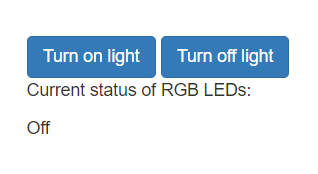
\includegraphics[scale=1]{Figures/remote_control.png}
    \caption{Interface for remote control of sensor network.}
    \label{fig:remote}
\end{figure}

\section{DynamoDB}
A second DynamoDB table was created to keep track of the status of the RGB LEDs for each of the nodes. This table uses only the device ID as the key. Every time an item is updated, the current value will be overwritten. This means that there will only be one query for each device at any time. This makes for a good way to keep data consistency throughout the system. The value to be posted is given by the POST request from the JavaScript function. 

The central device in the sensor network will continuously query the database for the status of each of the sensor nodes and updates them accordingly.  